
\section{Defined goal}\label{sec:defined-goal}
%**************************************************************

Most recent adversarial attack methods described in \ref{subsec:taxonomy-textual-adversarial-attacks} successfully decrease the accuracy of the target model.
However, since the main goal of the research is to enhance the robustness of the target model, we need to ensure that the quality of the crafted adversarial examples should be high, because the target model will be re-trained with them.

A successful natural language adversarial example can be defined as a perturbation that fools the model and fulfils  a set of linguistic constraints.
Using a sentiment analysis scenario as an example (Figure \ref{fig:3_adverarial_example}), an attacker can fool the system by changing only one word from “Perfect” to “Spotless” which can completely change the predicted output without being discerned by humans.


\begin{figure}[h]
  \centering
  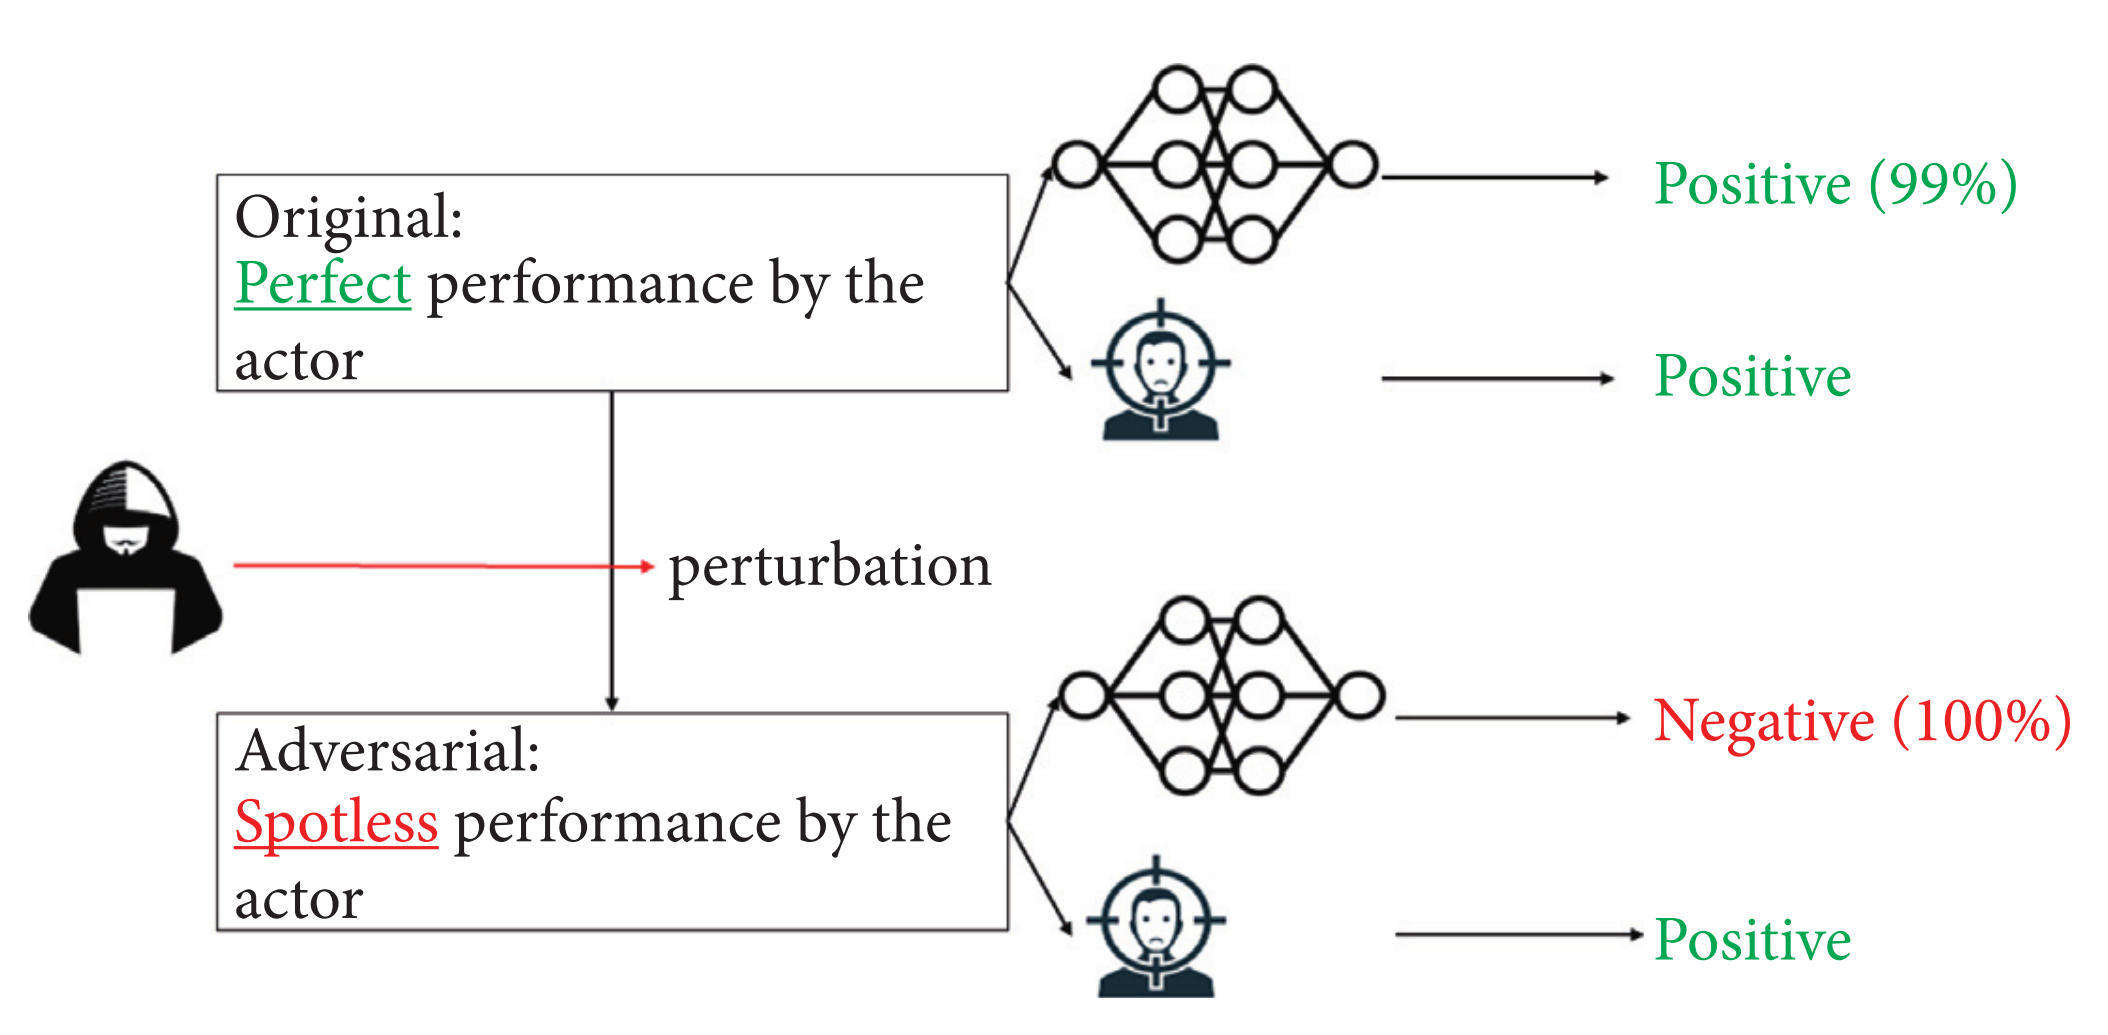
\includegraphics[width=0.7\linewidth]{images/3_adversarial_attack.png}
  \caption{Textual adversarial attack in sentiment analysis \cite{10.1155/2022/6458488}}
  \label{fig:3_adverarial_example}
\end{figure}

Formally, besides the ability to fool the target models, the outputs of a natural language attacking system should meet three key utility-preserving properties, defined by Jin et al. \cite{journals/corr/abs-1907-11932} as follows:
\begin{enumerate}
    \item \emph{human prediction consistency} - prediction by humans should remain unchanged;
    \item \emph{semantic similarity} -  the crafted example should bear the same meaning as the source, as judged by humans;
    \item \emph{language fluency} - generated examples should look natural and grammatical.
\end{enumerate}
%**************************************************************
\subsection{Problem to solve}\label{subsec:problem-to-solve}
Although attacks in NLP aspire to meet linguistic constraints, in practice, they frequently violate them.
Focusing on TextFooler and BERT-based attacks, they claim to create perturbations that preserve semantics, maintain grammaticality, and are not suspicious to readers. 
However, our inspection of the perturbations revealed that they violate these constraints.

On one hand, the perturbations generated by TextFooler solely account for the token level similarity via word embeddings, and not the overall sentence semantics. This can lead to out-of-context and unnaturally complex replacements.

On the other hand, with the capability of BERT, the perturbations crafted by BERT-based attacks are generated considering the context around. Therefore, the perturbations are fluent and reasonable.
Nevertheless, candidates generated from the masked language model can sometimes be antonyms or irrelevant to the original words, causing a semantic loss.

Table \ref{tab:3_1_wrong_adversarial_examples} highlights some examples of adversaries suffering from aforementioned issues.

\begin{table}[h]
    \footnotesize
    \centering
    \begin{tabularx}{\textwidth}{|l||l|X|}
      \hline
      \textbf{Method} & \textbf{Label}  & \textbf{Samples} \\
      \hline \hline
      \emph{TextFooler} & Original (\textcolor{ForestGreen}{POS}) & \textcolor{ForestGreen}{generates} an enormous \textcolor{ForestGreen}{feeling} of empathy for its \textcolor{ForestGreen}{characters} \\
                 & Perturbed (\textcolor{red}{NEG}) & \textcolor{red}{leeds} an enormous \textcolor{red}{foreboding} of empathy for its \textcolor{red}{fonts}
                 \\
      \hline
     
      \emph{BAE} & Original (\textcolor{red}{NEG}) & bears is even \textcolor{red}{worse} than i imagined a movie ever could be.     \\
      & Perturbed (\textcolor{ForestGreen}{POS}) & bears is even \textcolor{ForestGreen}{greater} than i imagined a movie ever could be.
    \\
        
      \hline
    \end{tabularx}
    \caption{Some adversarial samples generated with TextFooler and BAE}
  \label{tab:3_1_wrong_adversarial_examples}
\end{table}

%**************************************************************

\subsection{Research objective}\label{subsec:research-objective}

In order to address the research questions defined in Section \ref{sec:research-question}, 
we propose a new approach to generate adversarial examples that meet linguistic constraints.
In particular, we aim to demonstrate that:
\begin{itemize}
    \item using our evaluation framework defined in section \ref{sec:evaluation-framework}, we can identify the weaknesses of existing attack methods;
    \item the utility-preserving properties measured on the proposed solution outperform the state-of-the-art;
\end{itemize}
 

%**************************************************************